This chapter describes how we are to document and handle changes in regards to code. 

\subsection{Issues in GitLab}
In order to effectively distribute the work load across people in the different teams, issues in GitLab are to be used. This makes sure that we have a good overview of who is doing what during a specific time frame, what has the highest priority right now and so on. GitLab issues is to be found in GitLab in the left section. The issues works like a kanban board where some issues is to be done, some are under progress and some are finished and reviewed. The issues are have high or low priority regarding whether or not we believe them to be critical. The developers themselves are to select an issue that has a high priority if such an issue exists. 

The Kanban board for the development team is more elaborate since both developers and testers need to have a higher traceability of what requirement is being worked on and how to test the developed requirement. The first column in the board is where development leader Filip Eriksson adds issues that are directly linked to the requirements of the project. These issues shall include the number from the SRS so that the requirement issues are easily linked to the correct requirement in the SRS. The issues added shall also include a short description of what should be implemented to cover the requirement. The next step in the process is for testers to set up preliminary test case in order to implement test driven development. To use TDD, the different components in the web application needs to follow a naming convention, which is described in more detail in section \ref{Naming convention}. The development team then starts implementing the requirement based on their original plan and the test case done in step 2. When the requirement has been fully developed, the test is run to see that the requirement is successfully implemented. If the test succeeds, the issue shall be moved to "closed" and if not, it is to be moved back to implementation (development).


\begin{figure}[hbt!]
\centering
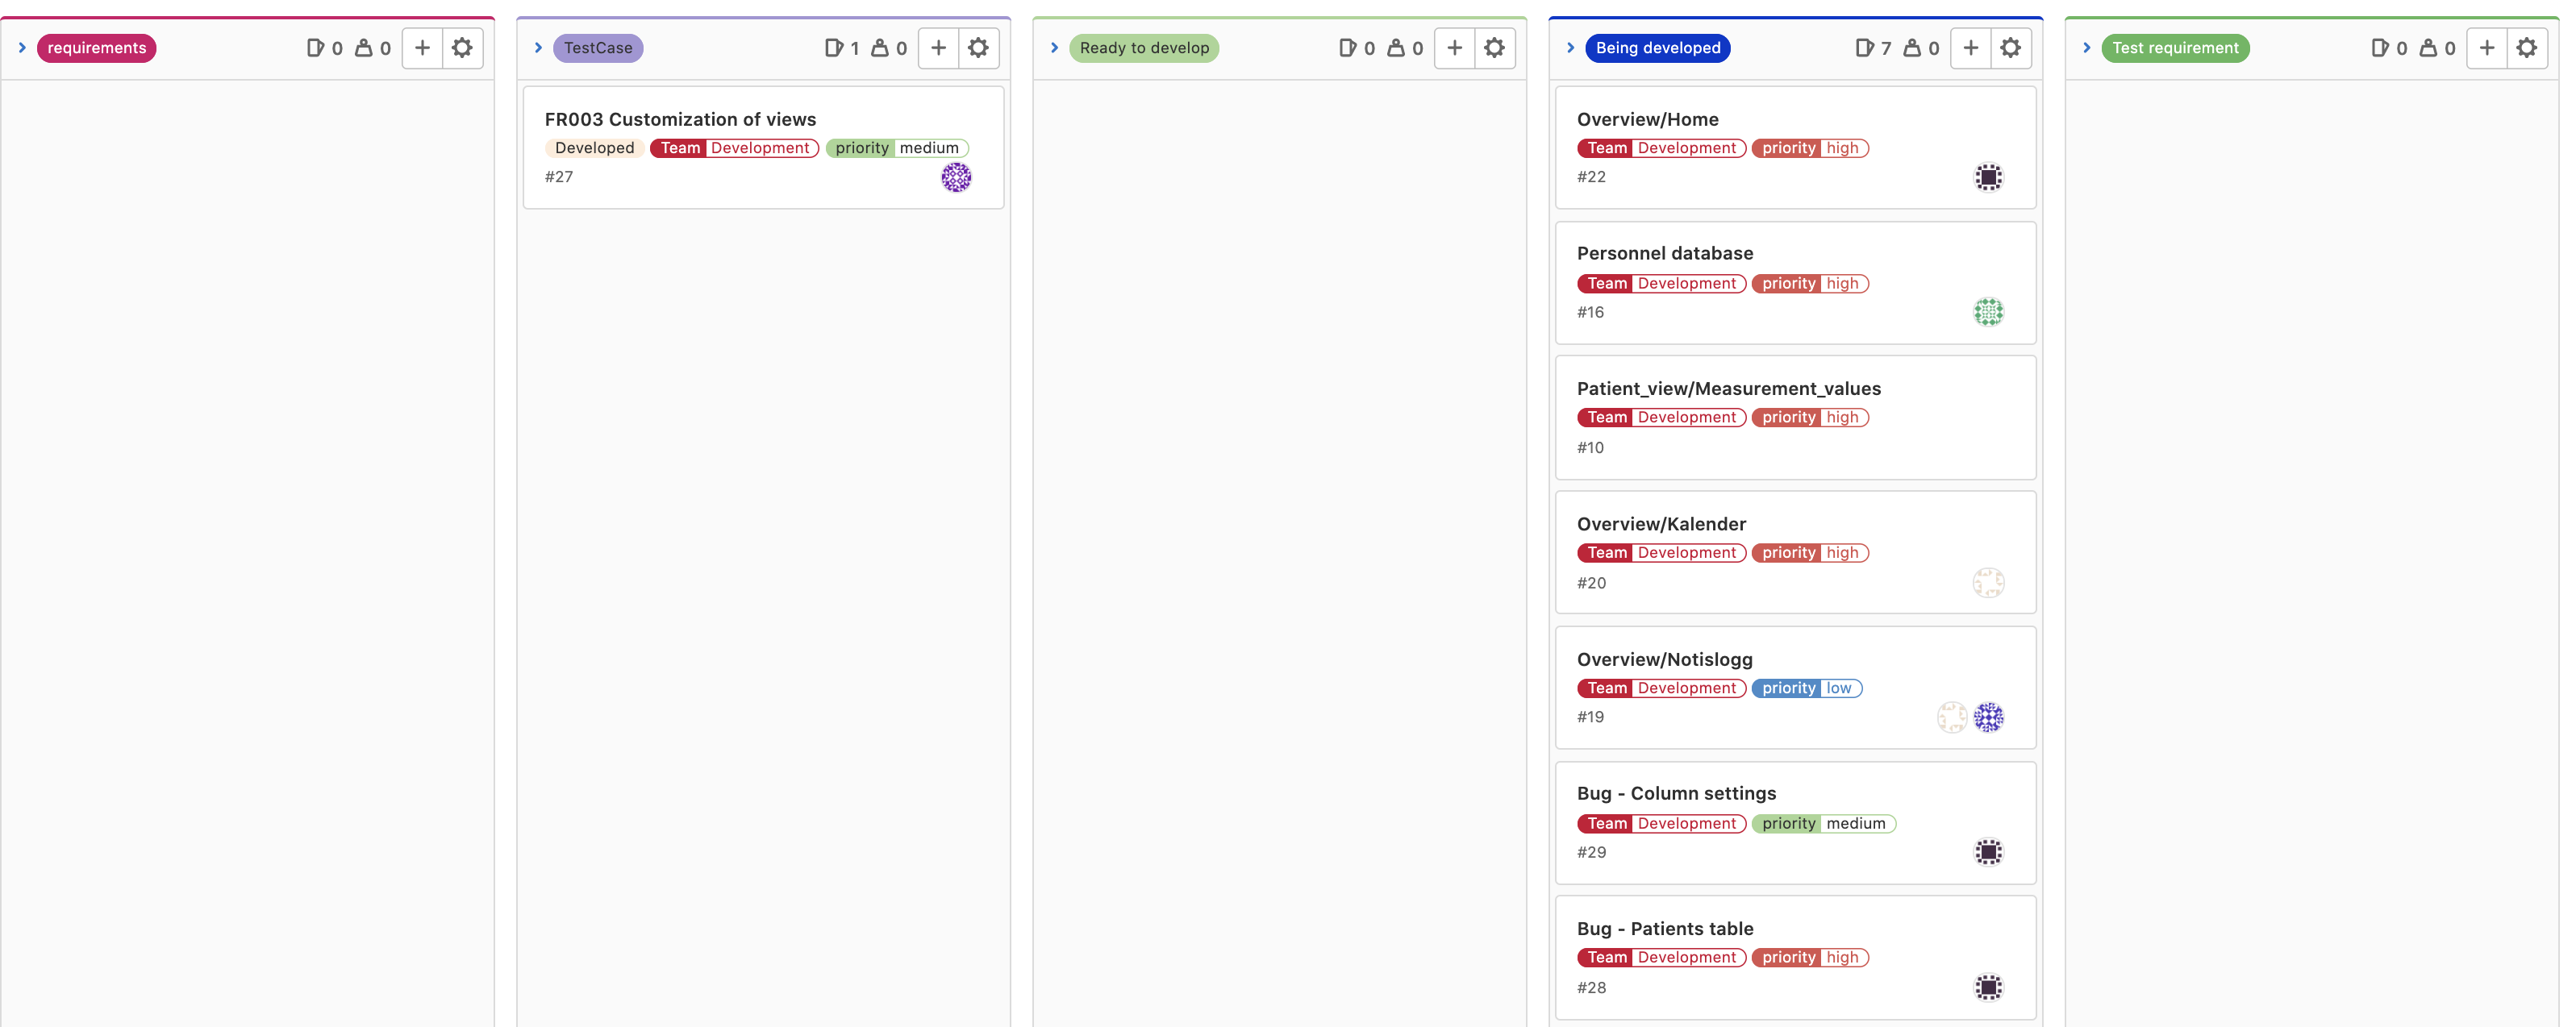
\includegraphics[width=15cm]{Kanbanboard.png}
\caption{Kanban Board for development and testing}
\label{fig:company structure}
\end{figure}


\subsection{Branches and Commits}
In this section, the processes for working with branches and what a commit should include is discussed in more detail. 

\subsubsection{Branches}
When working on a new feature for our software everything is to be done in a separate branch from our master. By working this way, we minimize the probability that something could go wrong with the master branch without anyone in the project group noticing it. When the software feature is done it is to be merged with master, but before the merge in accepted we run our continuous integration builds and tests. 

\textbf{Feature branches} that are directly branched from master should be named as follows: 
\begin{itemize}
    \item $<$Frontend\_implementation$>$
\end{itemize}
To clarify, we are going to have two groups of branches branched out from master. A new branch is therefore going to belong to either the front-end group or the back-end group. Merging of the Feature branches into master is going to be handled by Emil Strömberg. 



\subsubsection{Commits}
In order to have an easily read git repository history, commits should be done separately for every file that is commited, with a specific commit message for each file. Doing it this way makes it easier to track what work have been done to what file at a specific point in time. An example of a good commit message for a could be "Add patient table filling function". If you need to use "and" in your commit message, the commit includes too much new code or functionality.

\subsubsection{Comments in code}
When a subsub feature is merged with a sub feature, the code in the subsub feature must be well documented. This includes a summary of what the file is doing and how it works as well as more concrete information about every single function in the file. 

\subsubsection{READMEs}
To every new package that is created, a new readme file should also be created describing the functionality of the package as well as how it can be used. 



\subsection{CI/CD workflow}
We are to develop suitable unittests as well as automated web tests with Selenium, which is to be implemented in our CI-pipe. Our integrator Emil Strömberg has set up a basic CI-pipeline (as much as possible) and we're now able to perform continuous delivery. We are to work with continuous integration where we are to push our work to the child branch of master that we are working on after every work session. When the respective tasks are done they are to be merged with the master branch. As of now, we do not have any continuous delivery in our master branch since the backend branch is not yet ready. Getting the backend branch ready for continuous delivery is of high priority. When the back-end branch is ready, the backend and frontend branches are to be merged with master at least once every week. 

